%----------------------------------------------------------------------------------------
%	PACKAGES AND OTHER DOCUMENT CONFIGURATIONS
%----------------------------------------------------------------------------------------

\documentclass {article}
%
\usepackage[autostyle, italian=guillemets]{csquotes}
\usepackage[backend=biber]{biblatex}
%\usepackage{biblatex}
\addbibresource{biblio.bib}


\usepackage{blindtext} % Package to generate dummy text throughout this template 

\usepackage[sc]{mathpazo} % Use the Palatino font
\usepackage[T1]{fontenc} % Use 8-bit encoding that has 256 glyphs
\linespread{1.05} % Line spacing - Palatino needs more space between lines
\usepackage{microtype} % Slightly tweak font spacing for aesthetics

\usepackage[english]{babel} % Language hyphenation and typographical rules

\usepackage[hmarginratio=1:1,top=32mm,columnsep=20pt]{geometry} % Document margins
\usepackage[hang, small,labelfont=bf,up,textfont=it,up]{caption} % Custom captions under/above floats in tables or figures
\usepackage{booktabs} % Horizontal rules in tables

\usepackage{lettrine} % The lettrine is the first enlarged letter at the beginning of the text

\usepackage{enumitem} % Customized lists
\setlist[itemize]{noitemsep} % Make itemize lists more compact

\usepackage{abstract} % Allows abstract customization
\renewcommand{\abstractnamefont}{\normalfont\bfseries} % Set the "Abstract" text to bold
\renewcommand{\abstracttextfont}{\normalfont\small\itshape} % Set the abstract itself to small italic text

\usepackage{titlesec} % Allows customization of titles
%\renewcommand\thesection{\Roman{section}} % Roman numerals for the sections
%\renewcommand\thesubsection{\roman{subsection}} % roman numerals for subsections
\titleformat{\section}[block]{\large\scshape\centering}{\thesection.}{1em}{} % Change the look of the section titles
\titleformat{\subsection}[block]{\large}{\thesubsection.}{1em}{} % Change the look of the section titles

\usepackage{fancyhdr} % Headers and footers
\pagestyle{fancy} % All pages have headers and footers
\fancyhead{} % Blank out the default header
\fancyfoot{} % Blank out the default footer
\fancyhead[C]{Running title $\bullet$ February 2022 }%$\bullet$} % Custom header text
\fancyfoot[RO,LE]{\thepage} % Custom footer text

\usepackage{titling} % Customizing the title section

\usepackage{hyperref} % For hyperlinks in the PDF
\usepackage{graphicx}
\usepackage{amsmath} % questo serve per le matrici!
\hyphenpenalty=10000
\hbadness=10000

%----------------------------------------------------------------------------------------
%	TITLE SECTION
%----------------------------------------------------------------------------------------

\setlength{\droptitle}{-4\baselineskip} % Move the title up

\pretitle{\begin{center}\huge\bfseries} % Article title formatting
\posttitle{\end{center}} % Article title closing formatting
\title{Coupled Markov chains with applications to Approximate Bayesian Computation for model based clustering} % Article title
\author{%
\textsc{E. Bertoni, M. Caldarini, F. Di Filippo, G. Gabrielli, E. Musiari} \\[1ex] % Your name
\normalsize Politecnico di Milano \\ % Your institution
%\normalsize \href{mailto:john@smith.com}{john@smith.com} % Your email address
%\and % Uncomment if 2 authors are required, duplicate these 4 lines if more
%\textsc{Jane Smith}\thanks{Corresponding author} \\[1ex] % Second author's name
%\normalsize University of Utah \\ % Second author's institution
%\normalsize \href{mailto:jane@smith.com}{jane@smith.com} % Second author's email address
}
\date{\today} % Leave empty to omit a date
\renewcommand{\maketitlehookd}{%
\begin{abstract}
\noindent \blindtext % Dummy abstract text - replace \blindtext with your abstract text
\end{abstract}
}

%----------------------------------------------------------------------------------------

\begin{document}

% Print the title
\maketitle

%----------------------------------------------------------------------------------------
%	ARTICLE CONTENTS
%----------------------------------------------------------------------------------------

\section{Introduction}

\lettrine[nindent=0em,lines=3]{T}he aim of our project is to deal with two problems that can affect the same computation. The first one is to speed up Markov chain Monte Carlo (MCMC) methods using parallelization, while the second one is to manage the case in which the likelihood is computationally intractable. To solve the first problem, we used the Unbiased Markov chain Monte Carlo methods with couplings, instead for the second problem we used the Approximate Bayesian Computation.

%------------------------------------------------

\section{Methods}

%Parlare dei metodi di ABC e di Maximal coupling (con time average) in modo separato.
%
%poi parlare qua di come siano stati messi insieme o nella sezione dopo?

\subsection{Unbiased Markov chain Monte Carlo methods with couplings}


Markov chain Monte Carlo (MCMC) methods provide consistent approximations of high dimensional integrals, namely as the number of iterations goes to infinity. However, these estimators can be potentially biased for any fixed number of iterations, hence the aim is to propose a general construction to produce unbiased estimators of integrals with respect to a target probability distribution. 
The following results has been illustrated by Jacob, O'Leary and Atchadé in 2020 \cite{jacob2020}.

Glynn and Rhee \cite{glynn2014exact} illustrated a construction on Markov chains represented by iterated random functions; in their approach only two chains must be coupled for the proposed estimator to be unbiased, without further assumptions on the state space or target distribution. 
Indeed, we need an unbiased estimator in order to make the parallelization possible, that will lead to a faster computation of the MCMC.
%So the procedure consists in running 2 coupled Markov chains in each processor and the estimation is obtained calculating the mean of their convergence values.


Hence, the goal is to estimate
$$
\mathbb{E}_{\pi}[h(X)] 
= \int h(x) \pi (d x)
.
$$
The estimator is based on a coupled pair of Markov chains, $(X_t)_{t\geq 0}$ and $(Y_t)_{t\geq}$, which marginally start from $\pi_0$ and evolve accordingly to $P$.



Some assumptions must be considered:
\begin{enumerate}
	\item as $t \to \infty$, 
	$$ \mathbb E [h(X_t)] \to \mathbb E_\pi [h(X)];$$
	and there exists $\eta > 0$ and $D < \infty$ such that $\mathbb E [|h(X_t)|^{2 + \eta}] \leq D$ for all $t \geq 0$;
	
	
	\item the chains are such that the meeting time 
	$$
	\tau 
	= \inf\{t \geq 1 : X_t = Y_{t-1}\}
	$$ 
	satisfies $\mathbb{P}(\tau > t) \leq C \delta^t$ for all $t \geq 0$, for some constants $C < \infty$ and $\delta \in (0,1)$;
	
	
	\item the chains stay together after meeting:
	$$X_t = Y_{t-1} \quad  \forall t \geq \tau.$$
\end{enumerate}

Thanks to the previous assumptions it can be proved that:
%\begin{align*}
$$\mathbb{E}_{\pi}[h(X)] = \mathbb{E}[
h(X_k) + \sum_{t = k+1}^{\tau -1}\{h(X_t) - h(Y_{t-1})\} ]
;$$
%\end{align*}
and  the Rhee--Glynn estimator can be defined as:
$$ 
H_k(X,Y)
= h(X_k) + \sum_{t = k+1}^{\tau -1}\{h(X_t) - h(Y_{t-1})\} 
$$
which is unbiased by construction.




Time-averaged estimator can be considered as a special case of Rhee--Glynn estimator, in which $H_k(X,Y)$ can be computed for several values of $k$ from the same realization of the coupled chains, with unbiased average of them. It can used to allow computation, evaluated as:

$$
H_{k:m}(X,Y) = MCMC_{k:m} + BC_{k:m}
$$

where:
$$MCMC_{k:m}=\frac{1}{m-k+1}\sum_{l=k}^{m}h(X_l)$$  is the standard MCMC average;
 \small{$$BC_{k:m}=\sum_{l=k+1}^{\tau -1}\min(1, \frac{l-k}{m-k+1})\{h(X_l)-h(Y_{l-1})\} $$} is the bias correction;
 
 $m$ is the number of iterations, smaller than the case of a biased classical MCMC method; $k-1$ is the burn-in number; $\tau$ is a random variable for the meeting time.

The algorithm of the time-average estimator can be written as follows:
\begin{enumerate}
	\item draw $X_0$ and $Y_0$ from an initial distribution $\pi_0$ and draw $X_1 \sim P(X_0, \cdot)$;
	\item set $t=1$: while $t<\max\{m,\tau\}$ and:
	\begin{itemize}
		\item[a] draw $(X_{t+1}, Y_t)\sim \bar P \{(X_t, Y_{t-1}), \cdot \}$; %\textcolor{orange}{$\qquad \bar P$ must be evaluated before!}
		\item[b] set $t \leftarrow t+1$;
	\end{itemize}
	\item compute the time-averaged estimator:	 	$$
		H_{k:m}(X,Y)
		= \frac{1}{m-k+1}\sum_{l=k}^{m}h(X_l) $$
		$$
		+ \sum_{l=k+1}^{\tau -1}\min(1, \frac{l-k}{m-k+1})\{h(X_l)-h(Y_{l-1})\} .
		$$
	
\end{enumerate}
where $ \bar P$ must be evaluated before.


	Metropolis--Hasting algorithm allows the calculation of the coupled kernel $\bar P \{(X_t, Y_{t-1}), \cdot \}$:
	
	\begin{enumerate}
		\item sample $(X^\star, Y^\star) | (X_t, Y_{t-1})$ from a maximal coupling of $q(X_t, \cdot)$ and $q(Y_{t-1}, \cdot)$;
		\item sample $U \sim \mathcal{U}([0,1])$;
		\item if
		$$ U
		\leq \min\bigg \{
		1,
		\frac{ \pi(X^\star)q(X^\star,X_t)}{
			\pi(X_t)q(X_t, X^\star)}
		\bigg \}
		$$
		then $X_{t+1} = X^\star$; otherwise $X_t = X_{t-1}$;
		\item if
		$$ U
		\leq \min\bigg \{ 
		1,
		\frac{ \pi(Y^\star)q(Y^\star,Y_t)}{
			\pi(Y_t)q(Y_t, Y^\star)}
		\bigg \}
		$$
		then $Y_{t+1} = Y^\star$; otherwise $Y_t = Y_{t-1}$.
		
	\end{enumerate}

and it can be noticed that the acceptance conditions are based on the same samples from the uniform.

A maximal coupling between two distributions $p$ ad $q$ on a space $\mathcal{X}$ is a distribution of a pair of random variables$(X, \space Y)$ that maximizes $\mathbb{P}(X=Y)$, subject to the marginal constraints $X\sim p$ and $Y \sim q$ \cite{zhang2020markov} \cite{Cordaro2017past}.

We can proceed setting $p = \mathcal{N}(X_{t-1},1)$ and $q = \mathcal{N}(Y_{t-1},1)$, then:
\begin{enumerate}
	\item sample $X_t \sim p$;
	\item sample $W|X_t \sim \mathcal{U}\{[0,p(X_t)]\}$;
	\item if $W\leq q(X_t)$ then output $(X_t,X_t)$, otherwise:
	\begin{enumerate}
		\item sample $Y_t \sim q$;
		\item sample $W^\star | Y_t \sim \mathcal{U}\{[0, q(Y_t)]\}$ 
		until $W^\star > p(Y_t)$ and output $(X_t,Y_t)$.
	\end{enumerate}
\end{enumerate}
and hence the output follows a maximal coupling of $p$ and $q$. A complete discussion about this topic can be found in Rosenthal \cite{rosenthal1997faithful}.

Moreover, the absence of bias allows the application on time budget-constrained parallel simulation: independent unbiased estimators with finite variance can be generated on separate machines and combined into consistent and asymptotically normal estimators, leading to better results with respect to the non-parallelized version.

\subsubsection{Parallelized implementation results}
The unbiased Markov chain Monte Carlo method with couplings can be implemented allowing parallelization. Indeed, this method consist in generating many couples of chains, any couple can be given to a single core to be processed, instead of generating each couple sequentially.

To understand how to exploit the unbiasness of time-averaged estimator $H_{k:n}(X,Y)$ and how to find a criteria for settings parameters like number of iterations or number of chains, here we report some results.

Considering the assumptions of the method, for all $k\geq 0$ and $m \geq k$, the estimator $H_{k:m}(X,Y)$ has expectation $\mathbb{E}_\pi[h(X)]$, a finite variance and a finite computation time. This means that the mean of many $H_{k:m}(X,Y)$ converges to $\mathbb{E}_\pi[h(X)]$ as their number increases, thus we can sample many independent copies of $H_{k:n}(X,Y)$ in parallel and average the result to get a good approximation of $\mathbb{E}_\pi[h(X)]$.

In order to have a good estimation we have to consider also the variance of the estimation. Recall that we wrote the time-averaged estimator as the sum of the Markov chain Monte Carlo average and a bias correction: 
$$ 
H_{k:n}(X,Y) 
= MCMC_{k:m} + BC_{k:m},$$
thanks to that form we can write the estimator's variance as:
$$ 
\mathbb{V}[H_{k:m}(X,Y)] 
= \mathbb{E}[\{MCMC_{k_m} - \mathbb{E}_\pi[h(X)]\}^2] 
+ 2 \mathbb{E}[\{MCMC_{k:m} - \mathbb{E}[h(X)]\}BC_{k:m}] 
+ \mathbb{E}[BC_{k:m}^2] 
$$

We wrap the mean-square error:
$$
MSE_{k:m}=  \mathbb{E}[\{MCMC_{k_m} - \mathbb{E}_\pi[h(X)]\}^2],
$$
and, thanks to other results, we obtain the following bound for variance:
$$
\mathbb{V}[H_{k:m}(X,Y)]
\leq MSE_{k:m} + 2 \sqrt{MSE_{k:m} C(m,k)} + C(m,k)
$$
Where $C(m,k)$ is a function of $m$ and $k$ of the shape $\frac{A \, B^k}{m-k+1}$ where $A$ and $B$ are constants.

Therefore the variance is bounded by the mean-square error of the MCMC estimator plus additive therms that vanish polynomially in $m-k$.

Assuming that $m > \tau$ with large probability, it is proved that we can retrieve an asymptotic efficiency that is comparable with the underlying MCMC estimators with appropriate choices of $k$ and $m$ that depend on the distribution of the meeting time $\tau$.

In other words, the bias of the MCMC algorithm can be removed at the cost of an increased variance, which can in turn be reduced by choosing sufficiently large values of $k$ and $m$. This results in a trade-off with the desired level of parallelism: one might prefer to keep $k$ and $m$ small, yielding a suboptimal efficiency for $H_{k:m}(X,Y)$, but enabling more independent copies to be generated in a given computing time.


\subsection{Approximate Bayesian Computation}

Likelihood-free methods are used to solve the problem that concerns the intractable evaluation of the likelihood function. A way to solve this issue is to use Approximate Bayesian Computation method \cite{sisson2018overview}, in which samples are produced form an approximation of the posterios distribution.
Doing so the likelihood doesn't need to be evaluated in teh algorithm.

Our focus was on ABC-Markov chain Monte Carlo samplers using Metropolis–Hastings algorithm.

In the well known Metropolis–Hastings algorithm given the current chain state $\theta^{(i)}$, the next value is obtained by sampling a candidate value $\theta \,'$ from a proposal distribution $\theta' \sim g(\theta^{(i-1)},\theta)$, which is then accepted with probability
 $$ \alpha(\theta^{(i-1)},\theta')= \min  \{ 1, \frac{\pi(\theta'|y_obs)g(\theta',\theta^{(i-1)})}{\pi(\theta^{(i-1)}|y_obs)g(\theta^{(i-1)},\theta') } \} $$


Whereas the likelihood can't be evaluated, in the standard ABC computation the posterior is substituted with the approximated version $$\pi_{ABC}(\theta|s_obs) \propto \int K_h(\parallel s'-s_{obs}\parallel)Lik(\theta|s_obs)\pi(\theta) ds $$

where ${K_h(u)}  =  \frac{1}{h}  K \left( \frac{u}{h} \right)$ is the standard smoothing Kernel function of parameter $ h>0$,$ Lik(\theta|s_obs)$ is the intractable likelihood function and $s=S(y)$ is the low-dimensional vector of summary statistics.

Therefore we can rewrite the acceptance probability, after some semplification, as:
 $$ \alpha(\theta^{(i-1)},\theta')= \min  \{ 1, \frac{\pi_{ABC}(\theta'|s_{obs})g(\theta',\theta^{(i-1)})}{\pi_{ABC}(\theta^{(i-1)}|s_{obs})g(\theta^{(i-1)},\theta') } \} $$
 $$ =\min  \{ 1, \frac{\pi_{ABC}(K_h(\parallel s'-s_{obs}\parallel)   \pi(\theta')g(\theta',\theta^{(i-1)})}{K_h(\parallel s^{(i-1)}-s_{obs}\parallel)   \pi(\theta^{(i-1)})g(\theta^{(i-1)},\theta') } \} $$

sucht that there's no direct evaluation of the likelihood function.

A key task in this computation is to set efficiently both the scaling parameter h and the summary statistics:
the former parameter must be small to obtain the resulting estimate of the posterior closer to the true posterior. While the latter must be large enough to contain informations and low enough to avoid curse of dimensionality.
The best choice is to use sufficient statistics \cite{prangle2015summary}. As sufficient statistics can be much lower dimensional than the full dataset, it is clear that greater approximation accuracy can be achieved for the same computational overheads when using low dimensional statistics.
Then the comparison $\parallel y-y_{obs} \parallel$ might be replaced by $\parallel s-s_{obs} \parallel$ without too much loss of information, but with the advantage that the dimension of S(y) is now much lower.

%-----------------------
The algorithm \cite{fan2018abc} can be written as:

Input:
			\begin{itemize}
				\item a target posterior density $\pi(\theta | y_{obs}) \propto p(y_{obs}|\theta) \pi(\theta)$, consisting of a prior distribution $\pi(\theta)$ and a procedure of generating data under the model $p(y_{obs}|\theta)$;
				\item a proposal density $g(\theta' | \theta)$
				\item an integer $N \textgreater0$;
				\item a kernel function $K_h(u)$ and a scale parameter $h > 0$;
				\item a low dimensional vector of summary statistics $s=S(y)$.
			\end{itemize}
		
Initialize:
 Repeat until $$ K_h(\parallel s^{(0)}-s_{obs}\parallel) > 0$$ 
	\begin{enumerate}
		\item Choose an initial parameter vector $\theta_{(0)} \sim \pi(\theta)$ ;
		\item generate $ y^{(0)} \sim p(y|\theta^{(0)})$ from the model and compute summary statistics  $s^{(0)} = S(y^{(0)})$;
		
	\end{enumerate}


Sampling for $i=1,...,N$:
\begin{enumerate}
	\item generate candidate vector $\theta' \sim g(\theta^{(i-1)},\theta)$ from the proposal density $g$;
	\item generate $ y\,' \sim p(y|\theta')$ from the model and compute summary statistics  $s' = S(y\,')$;
	\item with probability $$\min \{ 1, \frac{K_h(\parallel s'-s_{obs}\parallel)   \pi(\theta')g(\theta',\theta^{(i-1)})}{K_h(\parallel s^{(i-1)}-s_{obs}\parallel)   \pi(\theta^{(i-1)})g(\theta^{(i-1)},\theta') } \}$$ 
	set $(\theta^{(i)},s^{(i)})=(	\theta',s')$. 
	Otherwise set  $(\theta^{(i)},s^{(i)})=(\theta^{(i-1)},s^{(i-1)})$.
\end{enumerate}

Output:

	 a set of correlated parameter vectors $\theta ^ {(1)},..., \theta ^ {(N)}$ from a Markov chain with stationary distribution $\pi_{ABC}(\theta |S_{obs})$.



%------------------------------------------------
\section{Implementation}

\subsection{Approximate Bayesian Computation}

\subsubsection{Univariate case}
The univariate ABC algorithm begins with generating 1000 samples from a Normal Distribution:
$$
	y_{obs} \sim  \mathcal{N} (\mu_{obs}, \sigma_{obs} ^2)
$$ 
and the chosen model is
$$
	y_{i} | \mu  \overset{iid}\sim \mathcal{N}(\mu, \sigma_{obs} ^2) \quad \text{for i=1,...,n}
$$
$$
	\mu  \sim \mathcal{N}(\mu_{0}, \sigma_{0}^2)
$$
with $ \sigma_{obs}$ known and $\mu_{0}, \sigma_{0} $ fixed.

The Gaussian Kernel function is
$$
	K(u) = \frac{1}{\sqrt{2\pi}} e^{-\frac{1}{2}u^2}
$$
The distance is the $L^2-$norm of the difference between $s_{0}$ and $s_{obs}$ and the summary statistics chosen are the sample mean and the vector of $9$ quantiles. Both of them are sufficient statistics.

\paragraph{First case:} sample mean\\
\begin{center} Input parameters: $\mu_{0}=8,\  \sigma_{0}^2=4,\  \mu_{obs}=10,\  \sigma_{obs}^2 =3,\ h=0.2$   \end{center}

\begin{figure}[h!]
	\centering
%	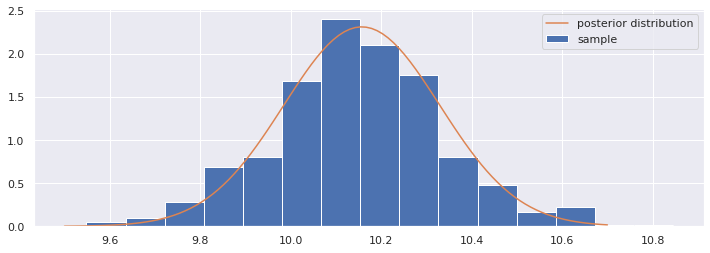
\includegraphics[width=\textwidth]{immagini_abc/h0.2}	
	\caption{}
	\label{abch02}
\end{figure}
\begin{figure}[h!]
	\centering
%	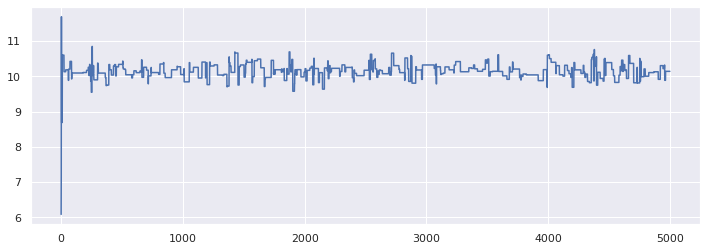
\includegraphics[width=\textwidth]{immagini_abc/sample0.2}	
	\caption{}
	\label{abcsample02}
\end{figure}


The posterior distribution has $\mu=10.151$ and $\sigma^2=0.0298$ \\

As mentioned in the chapter 2, the choice of parameter h is important.  \\
\begin{center} Input parameters: $\mu_{0}=8,\  \sigma_{0}^2=4,\  \mu_{obs}=10,\  \sigma_{obs}^2 =3,\ h=1.8$  \end{center}


\begin{figure}[h!]
	\centering
%	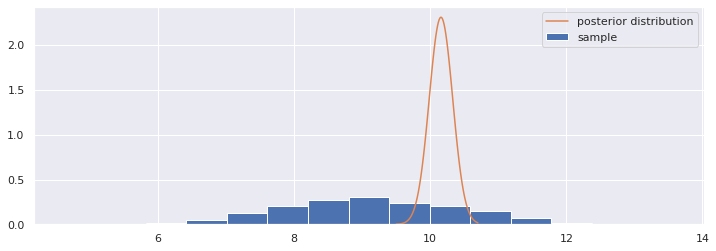
\includegraphics[width=\textwidth]{immagini_abc/h1.8}	
	\caption{}
	\label{abch18}
\end{figure}
\begin{figure}[h!]
	\centering
%	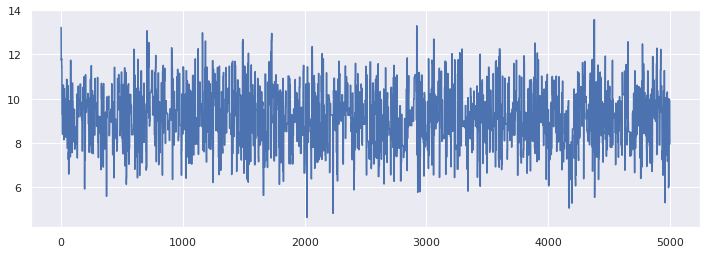
\includegraphics[width=\textwidth]{immagini_abc/sample1.8}	
	\caption{}
	\label{abch18}
\end{figure}


As seen in \ref{abch18}, a larger $h$ led to a poor approximation due to the acceptance of generated data that are far from the observed data.

\paragraph{Second case:} vector of 9 quantiles 
\begin{center} Input parameters: $\mu_{0}=8,\  \sigma_{0}^2=4,\  \mu_{obs}=10,\  \sigma_{obs}^2 =3,\ h=0.5$  \end{center}


\begin{figure}[h!]
	\centering
%	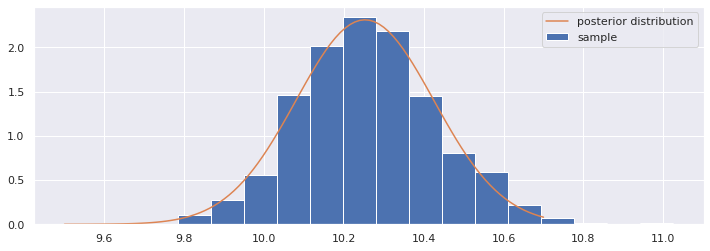
\includegraphics[width=\textwidth]{immagini_abc/S10.5}	
	\caption{}
	%\label{abch18}
\end{figure}
\begin{figure}[h!]
	\centering
%	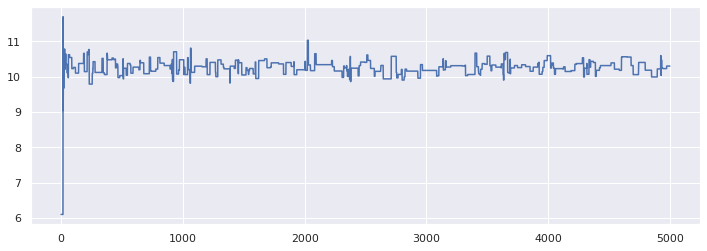
\includegraphics[width=\textwidth]{immagini_abc/sampleS10.5}	
	\caption{}
	%\label{abch18}
\end{figure}


The posterior distribution has $\mu=10.2527$ and $\sigma^2=0.0298$ 
\begin{center} Input parameters: $\mu_{0}=8,\  \sigma_{0}^2=4,\  \mu_{obs}=10,\  \sigma_{obs}^2 =3,\ h=1.8$  \end{center}
\begin{figure}[h!]
	\centering
%	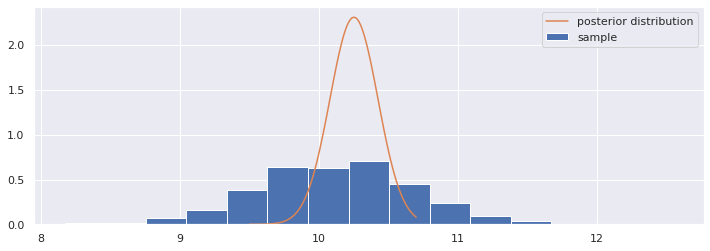
\includegraphics[width=\textwidth]{immagini_abc/S11.8}	
	\caption{}
	%\label{abch18}
\end{figure}
\begin{figure}[h!]
	\centering
%	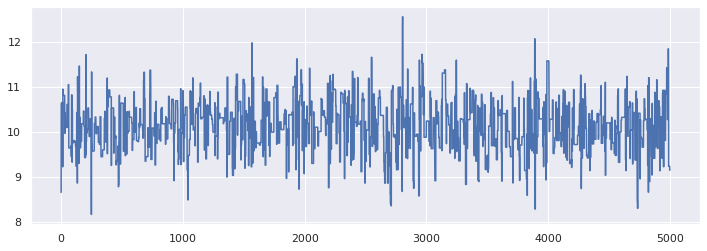
\includegraphics[width=\textwidth]{immagini_abc/sampleS11.8}	
	\caption{}
	%\label{abch18}
\end{figure}

\subsection{Multivariate case}
The multivariate ABC method is an extension of the univariate one. Samples has been generated from a Multivariate Normal Distribution.\\
The distance is the Mahalanobis distance between  $s_{0}$ and $s_{obs}$ and the summary statistic chosen is the sample mean.



\subsection{Unbiased Markov chain Monte Carlo methods with coupling}

\subsubsection{Univariate case}

The idea is to apply the method of coupling to a Metropolis-Hasting MCMC, obtaining two chains ${X_t}, \: {Y_t}$ that can be used to compute the time-average estimator $H_{k:m}(X,Y)$ defined above. In this way we can achieve an estimate of the unknow parameter \emph{k}.

As we said before, the principal idea of coupling is founding chains that meet in a finite time and remain together after the meeting. In order to do that, candidates can be generated with a maximal coupling algorithm, which maximizes the probability of getting two samples that are the same from two given distributions

During the computation of the time-averaged estimator we used  a Metropolis-Hastings algorithm to generate the pair of chains ${X_t}, \: {Y_t}$, computing 
$$ H_{k:m}(X,Y)
= \frac{1}{m-k+1}\sum_{l=k}^{m}h(X_l) 
+ \sum_{l=k+1}^{\tau -1}\min(1, \frac{l-k}{m-k+1})\{h(X_l)-h(Y_{l-1})\} 
$$
where \emph{m} is the maximum number of iterations, \emph{k} is the \emph{burnin} (namely the number of iterations that the chain needs to become stable) and $\tau$ is a random variable that represents the meeting time.

The computation of the Metropolis-Hastings algorithm is similar to the version with a singular chain, but we highlight that next iteration candidate pair is obtained from a maximal coupling.
Thanks to the fact that the time-averaged estimator is unbiased, we can parallelize the process running the algorithm on four different cores, putting together the estimates at the end, reducing the uncertainty. 

In our studies we set the model as:
$$ Y_i | \mu \sim{iid} \mathcal{N}(\mu, \sigma_{obs} ^2) \quad \text{for i= 1,...,n} $$
$$ \mu  \sim \mathcal{N}(\mu_0, \sigma_0^2)$$
with $\mu_0 = 8, \; \sigma^2_0 = 4$.
We generate $100$ samples from a Gaussian distribution:
$$
Y_{obs} \sim \mathcal{N}(\mu_{obs}, \sigma_{obs} ^2)
$$
with
$
\mu_{obs} = 10, \;
\sigma_{obs} ^2 = 3
$.

We obtained the posterior distribution:
$$  
	\mu | Y \sim \mathcal{N}(\mu_n, \sigma^2_n), 
	\quad \mu_n  \simeq 10.065,
	\quad \sigma^2_n \simeq 0.0298.
$$

The method has been implemented with the following setting, with parallelization:\\
Couples of chains: $4$;\\
Samples from each couple: $1000$;\\
Burnin: $100$.


Time Averaged Estimators mean obtained:
$$ 
	\mathbb{E}[H_{k:m}(X,Y)] = 10.042
$$
that is correctly close to the observed mean.
		
The results are graphically shown in the following plots.

	\begin{figure}[h!]
		\centering
		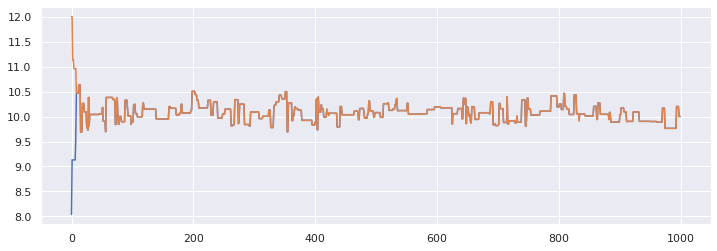
\includegraphics[width=\textwidth]{immagini_coupling/2_catene_coupling}	
		\caption{Coupled chains}
		\label{coupl1}
	\end{figure}

	\begin{figure}[h!]
		\centering
		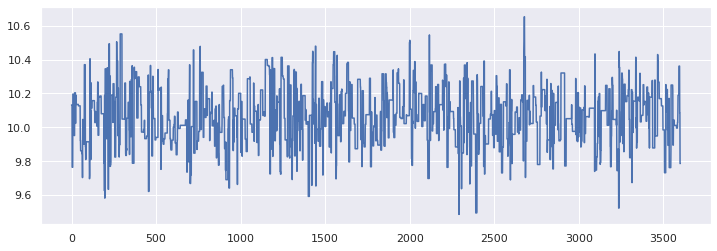
\includegraphics[width=\textwidth]{immagini_coupling/traceplot_coupling}
		\caption{Complete sampling}
		\label{coupl2}
	\end{figure}

	\begin{figure}[h!]
		\centering
		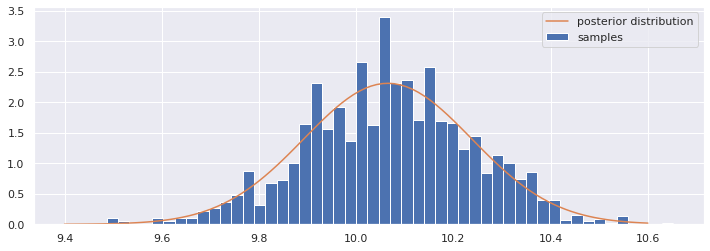
\includegraphics[width=\textwidth]{immagini_coupling/hist_coupling}
		\caption{Sampling histogram}
		\label{coupl3}
	\end{figure}


In figure \ref{coupl1} we can see that the chains meet after few iterations and remain together; in figure \ref{coupl3} we can notice that the posterior distribution is really closed to the theoretical one.

\newpage

\subsubsection{Multivariate case}

The univariate case can be easily extended to multivariate dimension, we used the following bivariate model:
$$ \boldsymbol{Y} | \boldsymbol{\mu} \overset{iid}{\sim} \mathcal{N}(\mu, \Sigma_{obs} ) \quad \text{for } i = 1 ... n $$
$$ \boldsymbol{\mu}  \sim \mathcal{N}(\mu_0, \sigma_0^2)$$
with $\boldsymbol{\mu}_0 =
\begin{Bmatrix}    % non so perchè non vada
12 \\
18
\end{Bmatrix} 
, \; \Sigma_0 = 3 \cdot \mathbb{I}$.

We generate $100$ samples from a Gaussian distribution:
$$
\boldsymbol{Y}_{obs} \sim \mathcal{N}(\boldsymbol{\mu}_{obs}, \Sigma_{obs})
$$
with
$  \boldsymbol{\mu}_{obs} =
\begin{Bmatrix}  
	10 \\
 	20
\end{Bmatrix}  
, \;  \Sigma_{obs}  = 5 \cdot \mathbb{I}
$.\\

The posterior distribution we obtain is as follows:
$$  \boldsymbol{\mu} | \boldsymbol{Y}_i \sim \mathcal{N}(\boldsymbol{\mu}_n, \Sigma_n), 
\quad \boldsymbol{\mu}_n \simeq \begin{Bmatrix}    % non so perchè non vada
10.103 \\
19.976
\end{Bmatrix} ,
\quad
\Sigma_n
\simeq 0.049 \cdot \mathbb{I} $$

The method has been implemented with the following setting, with parallelization:\\
Couples of chains: $4$;\\
Samples from each couple: $800$;\\
Burnin: $100$.



Time Averaged Estimators mean obtained:
$$ \mathbb{E}[H_{k:m}(\boldsymbol{X},\boldsymbol{Y})] \simeq \begin{Bmatrix}    % non so perchè non vada
10.008 \\
19.968
\end{Bmatrix}$$

Here the plot of the chains of the two variables, then the plots of the posterior sampling compared with the theoretical distribution::
\begin{figure}[h!]
	\centering
	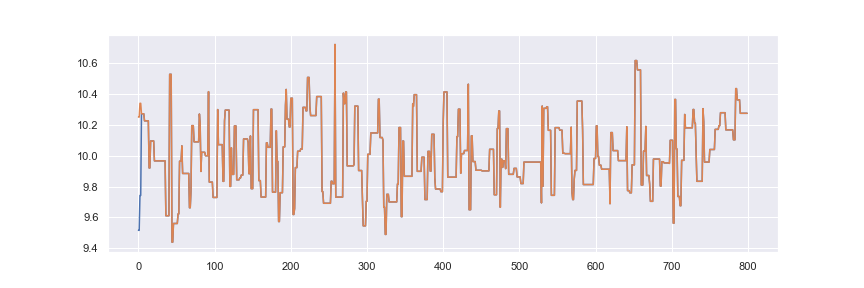
\includegraphics[width=\textwidth]{immagini_coupling_multivariate/coupling_mult_chain_meeeting_1}	
	\caption{First variable coupled chains}
\end{figure}

\begin{figure}[h!]
	\centering
	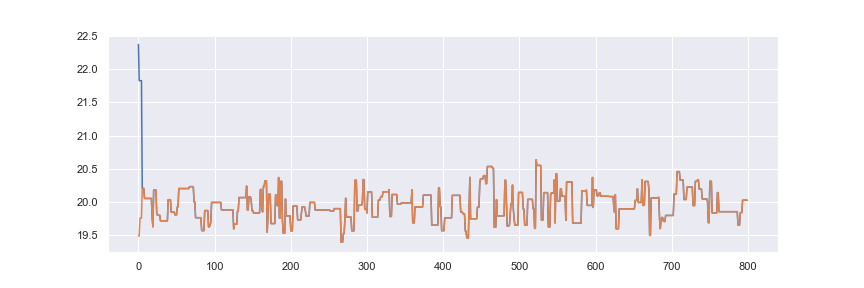
\includegraphics[width=\textwidth]{immagini_coupling_multivariate/coupling_mult_chain_meeeting_2}	
	\caption{Second variable coupled chains}
\end{figure}



\begin{figure}[h!]
	\centering
	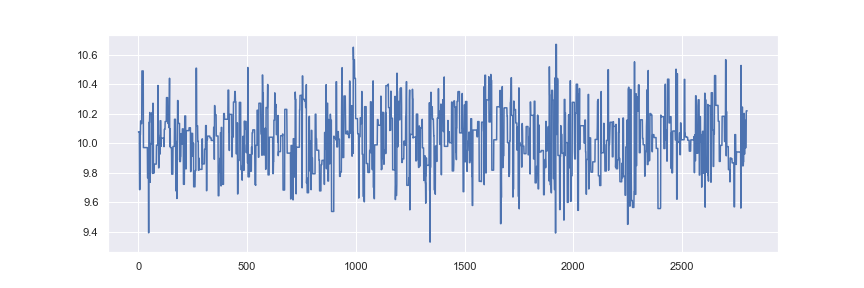
\includegraphics[width=\textwidth]{immagini_coupling_multivariate/coupling_mult_sampling_1}	
	\caption{First variable sampling (all chains together)}
\end{figure}
\begin{figure}[h!]
	\centering
	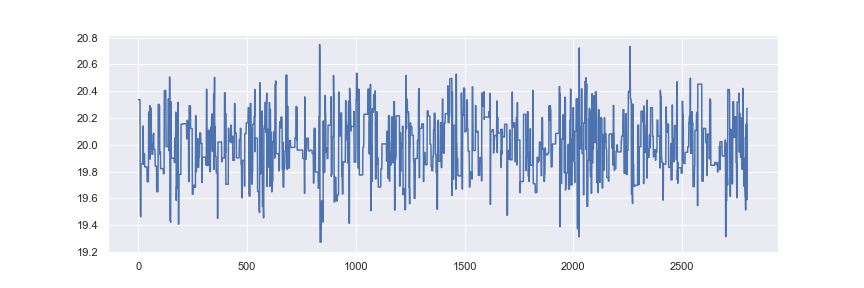
\includegraphics[width=\textwidth]{immagini_coupling_multivariate/coupling_mult_sampling_2}	
	\caption{Second variable sampling (all chains together)}
\end{figure}



\begin{figure}[h!]
	\centering
	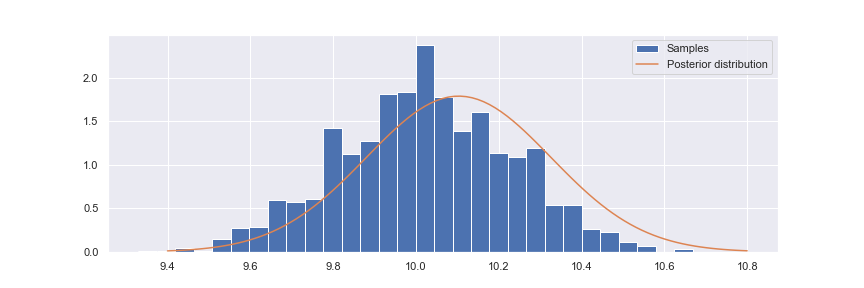
\includegraphics[width=\textwidth]{immagini_coupling_multivariate/coupling_mult_histogram_1}	
	\caption{First variable posterior}
\end{figure}
\begin{figure}[h!]
	\centering
	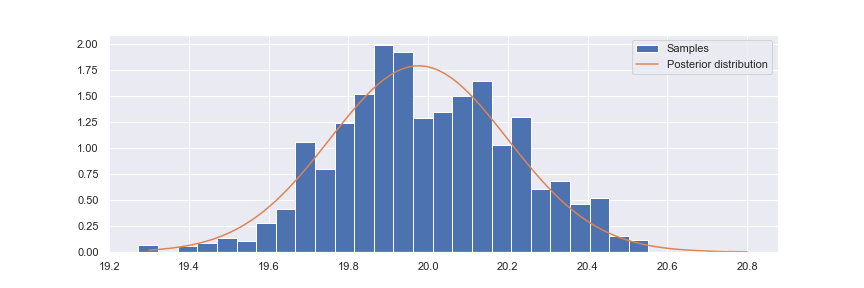
\includegraphics[width=\textwidth]{immagini_coupling_multivariate/coupling_mult_histogram_2}
	\caption{Second variable posterior}
\end{figure}

\clearpage

\subsubsection{Technicalities on parallel implementation}

In order to achieve parallelization, our choice is to use Python's standard package for parallelization, called multiprocessing (https://docs.python.org/3/library/multiprocessing.html). The Python's architecture does not allow multitreading parallelization, which would be optimal in terms of memory efficiency.

The main advantage of this technology is the possibility to have a full control of the process and the variable, but the main advantage consist of a limitation, in term of memory, of the data structure shared between processes. This limitation dumped on a trade-off between the number of coupled chain and the number of iterations: while this is acceptable for univariate sapling, such limits is too much limiting if sampling dimensionality is too high.

As we achieved the goal to parallelize the computation we do not attempt any other implementation, but there exist many other tools that can solve those issues and obtain a faster execution.

 
\clearpage

\subsection{The complete method}

\subsubsection{Univariate case with fixed variance}

We implemented an MCMC algorithm using Approximate Bayesian Computation to approximate the likelihood and Coupled Markov chanis.
The algorithm we computed: 

\begin{enumerate}
	\item Compute $s_{obs} = S(y_{obs})$;
	\item generate $\theta_{x}^{(0)} \sim  \pi(\mu)$ and $\theta_{y}^{(0)} \sim  \pi(\mu)$ from prior density;
	\item generate with a maximal coupling two samples of N observations such that $y_{1i} \sim \mathcal{N}(\theta_{x}^{(0)}, \sigma_{obs} ^2)$ and  $y_{2j} \sim \mathcal{N}(\theta_{y}^{(0)}, \sigma_{obs} ^2)$;
	\item compute $s_{x}^{(0)}=S(y_{1})$ and $s_{y}^{(0)}=S(y_{2})$;
	\item until $K_h(||s_{x}^{(0)}-s_{obs}||)>0$:
	\begin{itemize}
		\item generate $\theta_{x}^{(0)} \sim  \pi(\mu)$ from prior density;
		\item generate a sample of N observations such that $y_{1i} \sim \mathcal{N}(\theta_{x}^{(0)}, \sigma_{obs} ^2)$;
		\item compute $s_{x}^{(0)}=S(y_{1})$;
	\end{itemize}
	\item until $K_h(||s_{y}^{(0)}-s_{obs}||)>0$:
	\begin{itemize}
		\item generate $\theta_{y}^{(0)} \sim  \pi(\mu)$ from prior density;
		\item generate a sample of N observations such that $y_{2j} \sim \mathcal{N}(\theta_{y}^{(0)}, \sigma_{obs} ^2)$;
		\item compute $s_{y}^{(0)}=S(y_{2})$;
	\end{itemize}
	
\end{enumerate}


\begin{enumerate}
	\setcounter{enumi}{7}	
	
	\item for i = 1,...,N:
	\begin{itemize}
		\item generate [$\theta_{x}^{(i)},\theta_{y}^{(i)}$] from a maximal coupling given [$\theta_{x}^{(i-1)},\theta_{y}^{(i-1)}$];
		\item generate from a maximal coupling two samples of N observations $y_{1} \sim p(y|\theta_{x}^{(i)})$ and $y_{2} \sim p(y|\theta_{y}^{(i)})$;
		\item compute $s_{x}^{(i)}=S(y_{1})$ and $s_{y}^{(i)}=S(y_{2})$;
		\item accept $\theta_{x}^{(i)}$ with probability 
		$$
		\frac{
			K_h(||s_{x}^{(i)}-s_{obs}||)\pi(\theta_{x}^{(i)})
		}{
			K_h(||s_{x}^{(i-1)}-s_{obs}||)\pi(\theta_{x}^{(i-1)})
		}
		$$
		and accept $\theta_{y}^{(i)}$ with probability
		$$
		\frac{
			K_h(||s_{y}^{(i)}-s_{obs}||)\pi(\theta_{y}^{(i)})
		}{
			K_h(||s_{y}^{(i-1)}-s_{obs}||)\pi(\theta_{y}^{(i-1)})
		}.
		$$ 
	\end{itemize}
	
	
\end{enumerate}


As output: 
$$\theta_{x}^{(1)},...,\theta_{x}^{(N)}\sim \pi_{ABC} (\theta|y_{obs});$$
$$\theta_{y}^{(1)},...,\theta_{y}^{(N)} \sim \pi_{ABC} (\theta|y_{obs}).$$


\vspace{0.2cm}
We highlight that the key point is how each iteration works:
given the current values of $\theta$, a pair of candidates is generated from a maximal coupling; two samples of dimension \emph{n} are generated from the law of \emph{y} given $\theta$, maximizing the probability that the samples are the same;
the summary statistics is computed and the candidate $\theta_x ^{(i)}, \; \theta_y ^{(i)}$ are accepted with the \emph{Metropolis Hastings acceptance probability}. As output  we get two sets of parameter vectors of samples from the posterior distribution of $\theta$ given $S$.

In our study case, we used the sample mean as summary statistics, a $L^2-$norm as distance function and a Gaussian kernel function:
	$$
K(u) = 
\frac{1}{\sqrt{2\pi}} e^{-\frac{1}{2}u^2}, 
\quad K_h(u) 
= \frac{K(\frac u h)}{h}
$$ 

The model is the same as the above implementation: 
$$ Y_i | \mu \sim{iid} \mathcal{N}(\mu, \sigma_{obs} ^2) \quad \text{for i= 1,...,n} $$
$$ \mu  \sim \mathcal{N}(\mu_0, \sigma_0^2)$$
with $\mu_0 = 8, \; \sigma^2_0 = 4$.
We generate $n= 100$ samples from a Gaussian distribution:
$$
Y_{obs} \sim \mathcal{N}(\mu_{obs}, \sigma_{obs} ^2)
$$
with
$
\mu_{obs} = 10, \;
\sigma_{obs} ^2 = 3
$.

We obtained the posterior distribution:
$$  
\mu | Y \sim \mathcal{N}(\mu_n, \sigma^2_n), 
\quad \mu_n  \simeq 10.065,
\quad \sigma^2_n \simeq 0.0298.
$$
The results are shown in the following plots.
\begin{figure}[h!]
	%	{ \textbf{Coupled chains} }
	\centering
	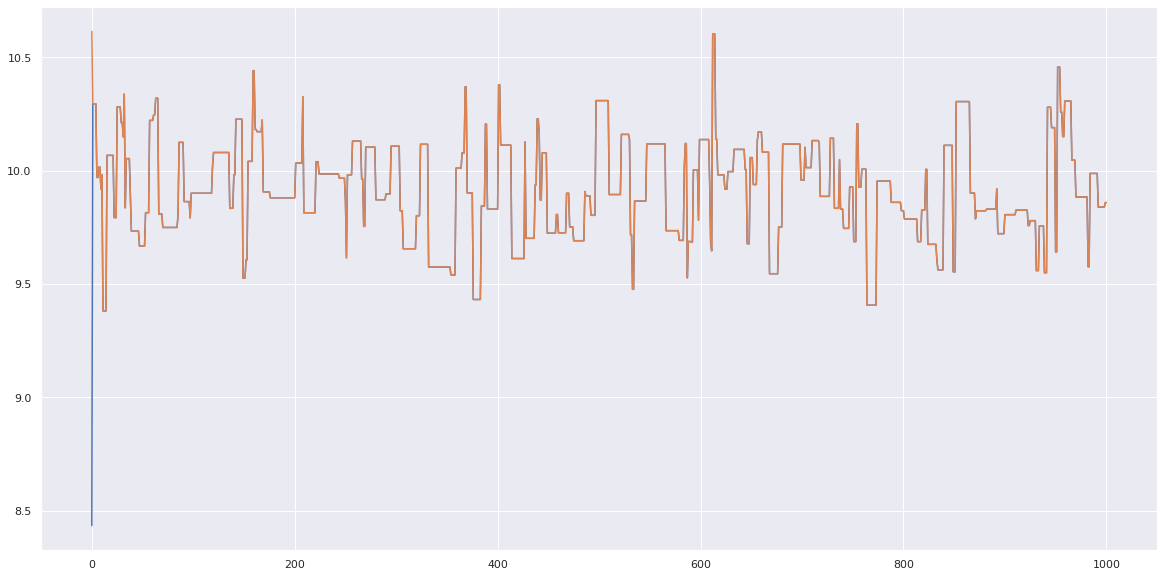
\includegraphics[width=\textwidth]{abc_coupling/2catabccoupling}	
	\caption{Coupled chains}
	\label{complete1}
	
\end{figure}

\begin{figure}[h!]
	%	{ %\textbf{Complete sampling}}
	\centering
	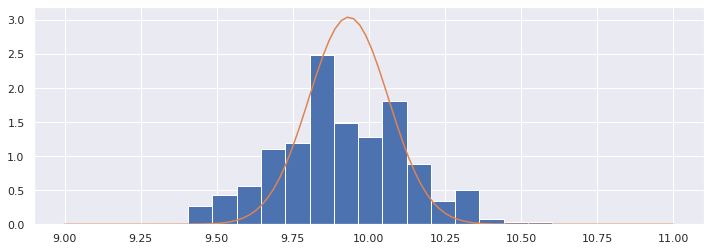
\includegraphics[width=\textwidth]{abc_coupling/histabccoupling}
	\caption{Sampling histogram with real distribution}   %without parallelization?
	\label{complete2}
\end{figure}

We can see in figure \ref{complete1} that the chains meet after few iterations remaining together while they converge to the posterior mean $\mu_{n}$. In figure \ref{complete2} we can see that our model approximates quite well the real distribution, even if the computation could be improved increasing the number of iterations performing a parallelization. %?



\subsubsection{Multivariate case with fixed variance}

The complete method can be easily extended to the multivariate version. We performed the same bivariate model that we used in the single multivariate coupling.
$$ \boldsymbol{Y} | \boldsymbol{\mu} \overset{iid}{\sim} \mathcal{N}(\mu, \Sigma_{obs} ) \quad \text{for } i = 1 ... n $$
$$ \boldsymbol{\mu}  \sim \mathcal{N}(\mu_0, \sigma_0^2)$$
with $\boldsymbol{\mu}_0 =
\begin{Bmatrix}    % non so perchè non vada
	12 \\
	18
\end{Bmatrix} 
, \; \Sigma_0 = 3 \cdot \mathbb{I}$.

We generate $100$ samples from a Gaussian distribution:
$$
\boldsymbol{Y}_{obs} \sim \mathcal{N}(\boldsymbol{\mu}_{obs}, \Sigma_{obs})
$$
with
$  \boldsymbol{\mu}_{obs} =
\begin{Bmatrix}  
	10 \\
	20
\end{Bmatrix}  
, \;  \Sigma_{obs}  = 5 \cdot \mathbb{I}
$.\\

The posterior distribution we obtain is as follows:
$$  \boldsymbol{\mu} | \boldsymbol{Y} \sim \mathcal{N}(\boldsymbol{\mu}_n, \Sigma_n), 
\quad \boldsymbol{\mu}_n \simeq \begin{Bmatrix}   
 % non so perchè non vada
9.556 \\
20.595
\end{Bmatrix} ,
\quad
\sigma^2_n
\simeq 0.050  $$
Time Averaged Estimators mean obtained:
$$ \mathbb{E}[H_{k:m}(\boldsymbol{X},\boldsymbol{Y})] \simeq \begin{Bmatrix}   
9.536 \\
20.551
\end{Bmatrix}$$

Here the plot of the chains of the two variables, then the plots of the posterior sampling compared with the theoretical distribution::
\begin{figure}[h!]
	\centering
	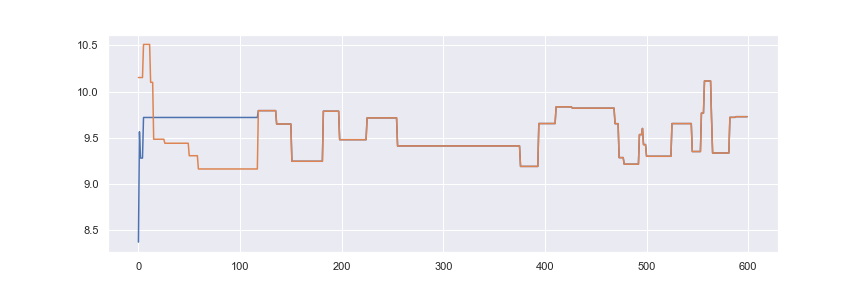
\includegraphics[width=\textwidth]{immagini_abc_coupling_multivariate/coupling_abc_mult_chain_meeeting_1}	
	\caption{First variable coupled chains}
\end{figure}
\begin{figure}[h!]
	\centering
	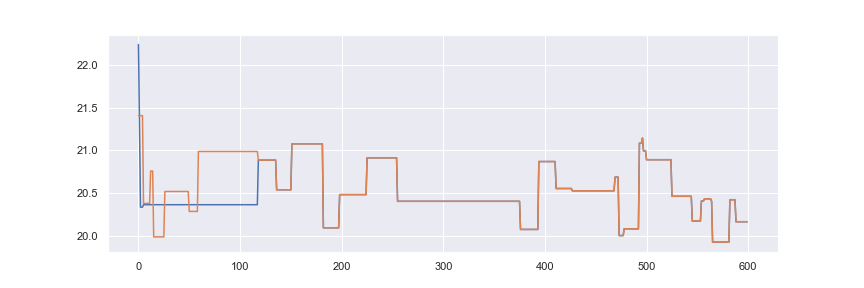
\includegraphics[width=\textwidth]{immagini_abc_coupling_multivariate/coupling_abc_mult_chain_meeeting_2}	
	\caption{Second variable coupled chains}
\end{figure}

\begin{figure}[h!]
	\centering
	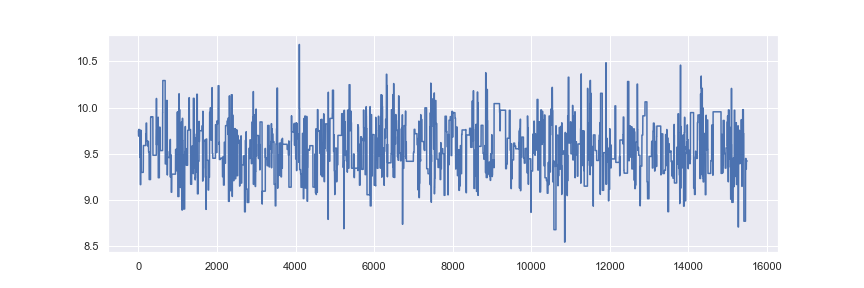
\includegraphics[width=\textwidth]{immagini_abc_coupling_multivariate/coupling_abc_mult_sampling_1}	
	\caption{First variable sampling (all chains together)}
\end{figure}
\begin{figure}[h!]
	\centering
	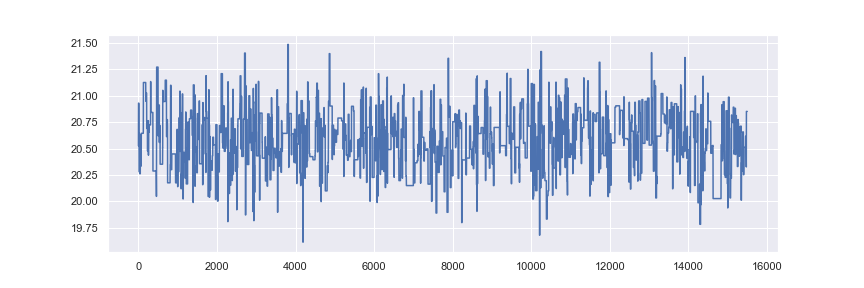
\includegraphics[width=\textwidth]{immagini_abc_coupling_multivariate/coupling_abc_mult_sampling_2}	
	\caption{Second variable sampling (all chains together)}
\end{figure}

\begin{figure}[h!]
	\centering
	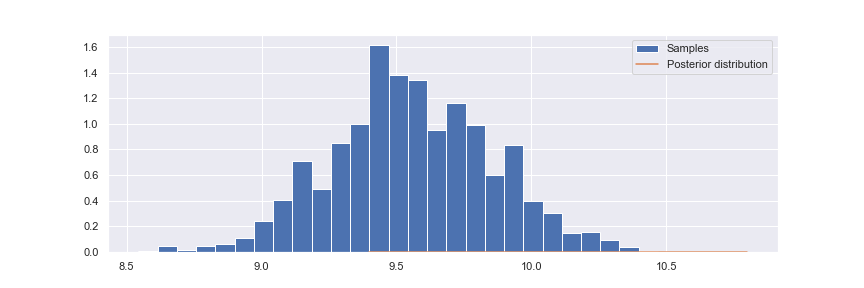
\includegraphics[width=\textwidth]{immagini_abc_coupling_multivariate/coupling_abc_mult_histogram_1}	
	\caption{First variable posterior}
\end{figure}
\begin{figure}[h!]
	\centering
	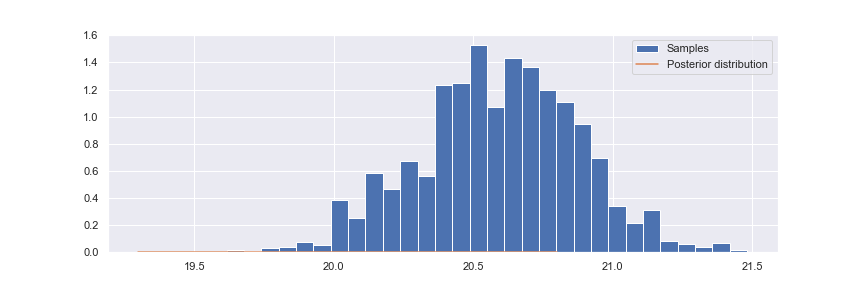
\includegraphics[width=\textwidth]{immagini_abc_coupling_multivariate/coupling_abc_mult_histogram_2}	
	\caption{Second variable posterior}
\end{figure}



\subsubsection{Univariate case with both mean and variance unknown}

This is also an extension of the Univariate case with fixed variance where $\theta = (\mu,\sigma)$

We assume as model:
$$ Y_i | \mu \sim{iid} \mathcal{N}(\mu, \sigma ^2) \quad \text{for i= 1,...,n} $$
$$ \mu  \sim \mathcal{N}(\mu_0, \sigma_0^2)$$
$$ \sigma^2 \sim InvGa(a_0,b_0)
$$
with $\mu_0=8, \sigma_0^2=4$ and $a_0=1, b_0=1$.

We generate $n= 100$ samples from a Gaussian distribution:
$$
Y_{obs} \sim \mathcal{N}(\mu_{obs}, \sigma_{obs} ^2)
$$
with
$
\mu_{obs} = 10, \;
\sigma_{obs} ^2 = 3
$.
As sufficient summary statistics we set (sample mean, sample variance), a $L^2-$norm as distance function and a Gaussian kernel function with scaling parameter h = 0.3 

The method has been implemented with the following setting, with parallelization:\\
Couples of chains: $4$;\\
Samples from each couple: $1000$;\\
Burnin: $100$.

For the MH ABC and coupled MCMC algorithm we define as proposal distribution for the parameters' update:
\begin{center}
	$ \mu^{i+1} \sim	\mathcal{N}( \mu^{i}, 0.1^2) $
	
	$ log(\sigma^{2(i+1)}) \sim \mathcal{N}( log(\sigma^{2(i)}), 0.1^2) $
\end{center}
the logarithm trasformation is needed to keep the proposed value of $ \sigma^2$ within its domain, 
which is $\mathbb{R^{+}}$


	
\textbf{Posterior}:
It would be impossible to compute the marginal posterior distribution, thus we obtain the conditional posterior distribution, or full conditional distributions:
Given $\mathbf{y} \in \mathbb{R^{n}} $

	
	$$ \mu| \sigma^2,\mathbf{y} \sim	\mathcal{N}( \sigma_n\mu_n, \sigma_n^2) $$
	
	$$ \sigma^{2} \mu,\mathbf{y} \sim InvGa( a_n,b_n)$$
	
	where $ \mu_n= n\bar y/\sigma_0^2 + \mu_0/\sigma_0^2$
		
and $a_n= a + n/2n=2, \  b_n=b + n\frac{(\mu-\bar y)^2}{2} +	\frac{\sum_{i=1}^n (y-\bar y)^2}2{} $


\textbf{Results}:
Time Averaged Estimators mean obtained:
$$ \mathbb{E}[H_{k:m}(X_{\mu}, Y_{\mu})] \simeq 9.8   % non so perchè non vada
$$
$$ \mathbb{E}[H_{k:m}(X_{\sigma^2}, Y_{\sigma^2})] \simeq 2.56   % non so perchè non vada
$$


As seen in the plots \ref{mucoupledchains} and \ref{sigmacoupledchains} coupled chains meet after few iterations.
In \ref{muhistdouble} and \ref{sigmahistdouble} we can observe the sampled posterior distribution and the estimated one.


%----- MU ---------
\begin{figure}[h!]
	%	{ %\textbf{Complete sampling}}
	\centering
	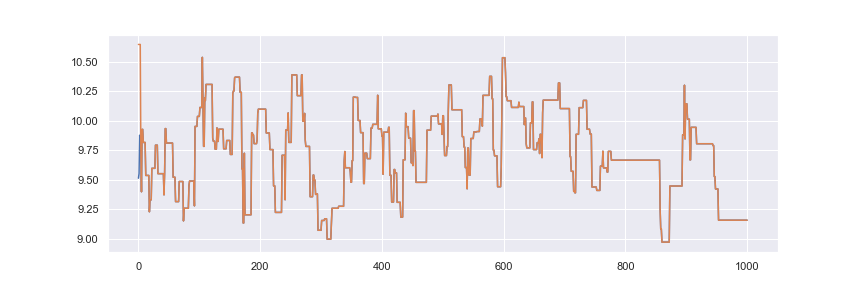
\includegraphics[width=\textwidth]{doublecoupling_pack/doublecoupling_mu_chain_meeting}
	\caption{Coupled chains for parameter $\mu$ }   %without parallelization?
	\label{mucoupledchains}
\end{figure}

\begin{figure}[h!]
	%	{ %\textbf{Complete sampling}}
	\centering
	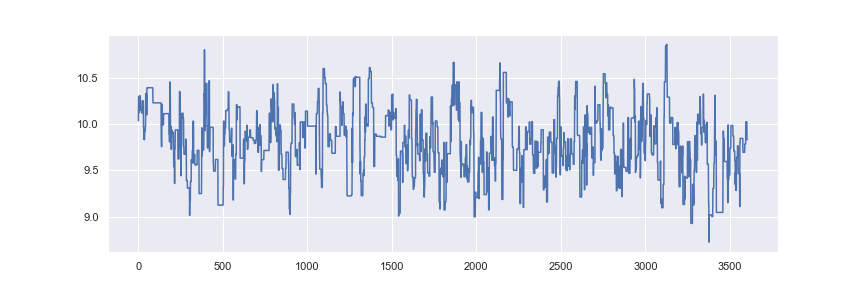
\includegraphics[width=\textwidth]{doublecoupling_pack/doublecoupling_sampling_mu}
	\caption{Sampling from all accepted parallelized chains for parameter $\mu$ }   %without parallelization?
	\label{muallsamdouble}
\end{figure}


\begin{figure}[h!]
	%	{ %\textbf{Complete sampling}}
	\centering
	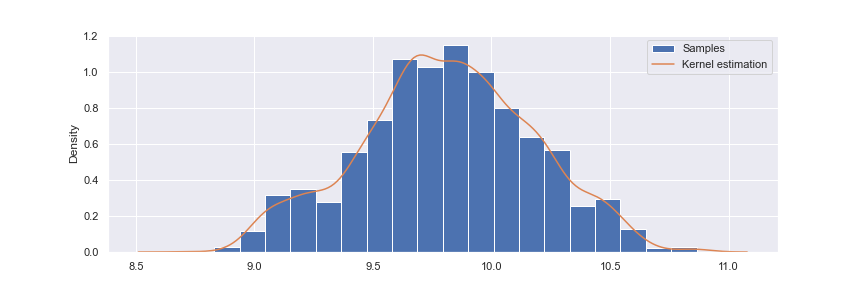
\includegraphics[width=\textwidth]{doublecoupling_pack/doublecoupling_mu_histogram_kernel}
	\caption{Histogram for parameter $\mu$: Sampling from all accepted parallelized chains with estimated kernel }   %without parallelization?
	\label{muhistdouble}
\end{figure}






%---- SIGMA ---
\begin{figure}[h!]
	%	{ %\textbf{Complete sampling}}
	\centering
	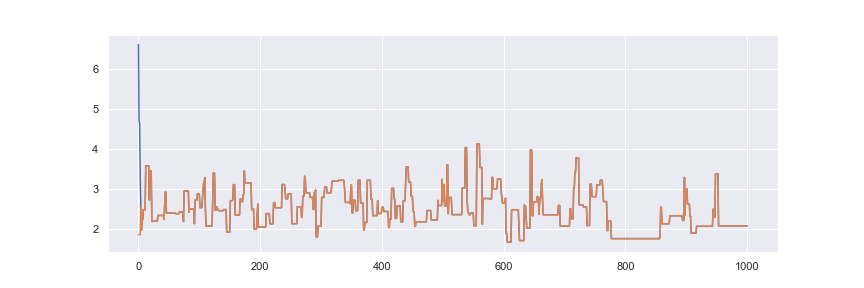
\includegraphics[width=\textwidth]{doublecoupling_pack/doublecoupling_sigma_chain_meeting}
	\caption{Coupled chains for parameter $\sigma^2$ }   %without parallelization?
	\label{sigmacoupledchains}
\end{figure}

\begin{figure}[h!]
	%	{ %\textbf{Complete sampling}}
	\centering
	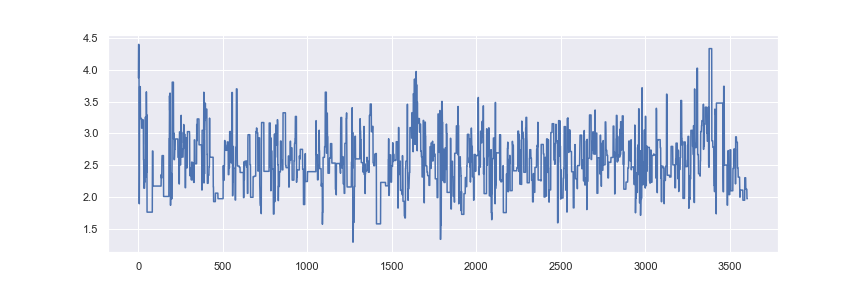
\includegraphics[width=\textwidth]{doublecoupling_pack/doublecoupling_sampling_sigma}
	\caption{Sampling from all accepted parallelized chains for parameter $\sigma^2$ }   %without parallelization?
	\label{sigmaallsamdouble}
\end{figure}


\begin{figure}[h!]
	%	{ %\textbf{Complete sampling}}
	\centering
	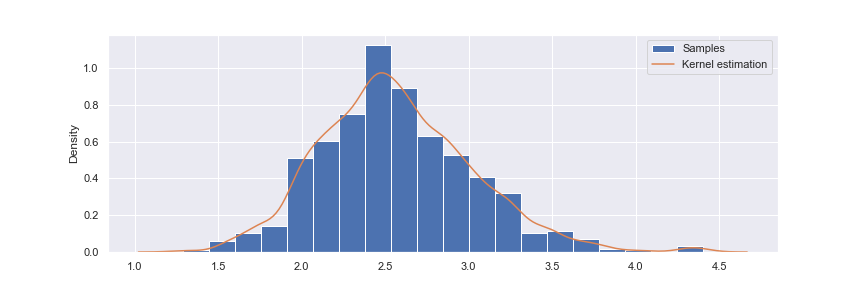
\includegraphics[width=\textwidth]{doublecoupling_pack/doublecoupling_sigma_histogram_kernel}
	\caption{Histogram for parameter $\sigma^2$: Sampling from all accepted parallelized chains with estimated kernel }   %without parallelization?
	\label{sigmahistdouble}
\end{figure}














	\section{Numerical Experiments}
In order to test our method on a more complex problem, we followed the common numerical experiment in the literature: ABC applied on the g-and-k distribution.
The goal is to, not only, apply ABC algorithm to this problem, but also the Unbiased coupled Markov chain Monte Carlo method.


\subsection{Univariate g-and-k distribution}

A classical numerical experiments in the ABC literature is to test the algorithm on the univariate g-and-k distribution.
The likelihood is intractable, therefore the distribution is defined in terms of its quantile function:

\begin{center}
	
	$$ r \in (0,1) \longmapsto   a + b (1+0.8\left(\frac{1-exp(-g \cdot z(r))}{1+exp(-g\cdot z(r))}\right)(1+ z(r)^{2})^k\cdot z(r)  $$
\end{center}



where $z(r)$ is the r-th quantile of the standard Normal distribution,
while a and b are location and scale parameters and g and k are related to skewness and kurtosis.
%Skewness is a measure of symmetry, or more precisely, the lack of symmetry. ... Kurtosis is a measure of whether the data are heavy-tailed or light-tailed relative to a normal distribution. That is, data sets with high kurtosis tend to have heavy tails, or outliers


Sampling from this distribution can be done by generating $z(r)$s as samples from a $\mathcal{N}(0,1)$: 
$z(r) \sim \mathcal{N}(0,1)$

To complete the model we assume prior probability distribution as follows:
\begin{center}
	$ a \sim \mathcal{U}([0,10])$
	
	$ b \sim \mathcal{U}([0,10])$
	
	$ g \sim \mathcal{U}([0,10])$
	
	$ k \sim \mathcal{U}([0,10])$
\end{center}


To test this distribution we sampled a set of observation $y_{obs}$ imposing the following values to the parameters, following the path of Jacob et al.:

a=3, b=1, g=2, k=0.5

A key point in the ABC procedure is the decision of the summary statistics, which in this case, are taken as the 10 equidistant quantiles as well as the minimum.

As before we set 

\textbf{Distance}: 
$$L^2-norm\ of\ the\ difference\ of\ S(y)\ and\ s_{obs}$$
%malanobis nel multivariato

\textbf{Kernel function}: 
$$
K(u) = 
\frac{1}{\sqrt{2\pi}} e^{-\frac{1}{2}u^2}, 
\quad K_h(u) 
= \frac{K(\frac u h)}{h}
$$



%\subsection{ABC and coupled Markov chain Monte Carlo method: inference on one parameter}
%
%Parameters b,g,k are fixed equal to the observation parameters, while parameter a is random
%The model is the one explained above.
%\begin{enumerate}
%\item Initialization:
%$$ a_{1}^{(0)} \sim \mathcal{U}([0,10])$$
%
%$$ a_{2}^{(0)} \sim \mathcal{U}([0,10])$$
%
%\item for k in (1,2):
%for j in (1,...,$n_{obs}$):
%\begin{itemize}
%	\item $z^{(0,j)}(r) \sim \mathcal{N}(0,1)  $
%	
%	\item $ y_{k}^{(0,j)} \sim quantile function(z^{(0,j)}(r))$
%	
%	\item compute $ s_{k}^{(0)} =S(y_{k}^{(0)})$
%\end{itemize}
%for j in (1,...,$n_{obs}$):
%
%Until $Kh(\|s_{1}^{(0)} - s_{obs}\|)>0$:
%\begin{enumerate}
%	\item Generate $a_{1}^{(0)} \sim \mathcal{U}([0,10])$ from prior density.
%	\item Generate $z_{1}^{(0)}(r) \sim \mathcal{N}(0,1)$
%	\item Generate a sample of 1000 observations such that $y_{1} \sim quantile function(z_{1}^{(0)}(r),a_{1}^{0})$
%	\item Compute $s_{1}^{(0)}=S(y_{1})$
%	
%\end{enumerate}
%Untill $Kh(\|s_{2}^{(0)} - s_{obs}\|)>0$:
%\begin{enumerate}
%	\item Generate $a_{2}^{(0)} \sim \mathcal{U}([0,10])$ from prior density.
%	\item Generate $z_{2}^{(0)}(r) \sim \mathcal{N}(0,1)$
%	\item Generate a sample of 1000 observations such that $y_{2} \sim quantile function(z_{2}^{(0)}(r),a_{2}^{(0)})$
%	\item Compute $s_{2}^{(0)}=S(y_{2})$
%\end{enumerate}
%
%
%for i in (1,...,M):
%\begin{enumerate}
%	\item 	generate $a_{1}^{(i)},a_{2}^{(i)}$  from maximalcoupling$(a_{1}^{(i-1)},a_{2}^{(i-1)})$
%	
%	for j in (1,...,n):
%	\begin{itemize}
%		\item $z^{(i,j)}(r) \sim \mathcal{N}(0,1)$
%		\item generate:
%		$ y_{1}^{(ij)} \sim quantile function(z^{(i,j)}(r), \theta^{(i-1)})$
%		$ y_{2}^{(ij)} \sim quantile function(z^{(i,j)}(r), \theta^{(i-1)})$
%		
%	\end{itemize}
%	
%	\item Compute the summaries  $ s_{1}^{(i)} =S(y_{1}^{(i)})$ and $ s_{2}^{(i)} =S(y_{2}^{(i)})$
%	
%	
%	\item acceptance:
%	\begin{itemize}
%		\item Accept $a_{1}^{(i)}$ with probability $\frac{Kh(\|s_{1}^{(i)}-s_{obs}\|)\pi(a_{1}^{(i)})}{Kh(\|s_{1}^{(i-1)}- s_{obs}\|)\pi(a_{1}^{(i-1)})} $   otherwise $a_{1}^{(i)}=a_{1}^{(i-1)}$
%		
%		\item Accept $a_{2}^{(i)}$ with probability $\frac{Kh(\|s_{2}^{(i)}-s_{obs}\|)\pi(a_{2}^{(i)})}{Kh(\|s_{2}^{(i-1)}-s_{obs}\|)\pi(a_{2}^{(i-1)})} $  otherwise $  a_{2}^{(i)}=a_{2}^{(i-1)}$
%	\end{itemize}
%\end{enumerate}
%
%\end{enumerate}



\subsubsection{ABC and coupled Markov chain Monte Carlo method}
given $\theta =( a,b,g,k )$
\begin{enumerate}

\item Initialization:
for k in (1,2):
$ \theta_{k}^{(0)} \sim \mathcal{U}([0,10]^4)$ 

\begin{itemize}
\item for j in (1,...,$n_{obs}$):
\begin{itemize}
	\item $z^{(0,j)}(r) \sim \mathcal{N}(0,1)  $
	
	\item $ y_{k}^{(0,j)} \sim quantilefunction(z^{(0,j)}(r),\theta_{k}^{(0)})$
	
	\item compute $ s_{k}^{(0)} =S(y_{k}^{(0)})$
\end{itemize}

\item Untill $Kh(\|s_{k}^{(0)} - s_{obs}\|)>0$:
\begin{itemize}
	\item Generate $\theta_{k}^{(0)} \sim \mathcal{U}([0,10]^4)$ from prior density.
	\item Generate $z^{(0)}(r) \sim \mathcal{N}(0,1)$
	\item Generate a sample of 1000 observations such that $y_{k} \sim quantile function(z{(0)}(r),\theta_{k}^{0})$
	\item Compute $s_{k}^{(0)}=S(y_{k})$
	
\end{itemize}
\end{itemize}


\item for i in (1,...,M):
\begin{itemize}
	\item 	generate $\theta_{1}^{(i)},\theta_{2}^{(i)}$  from maximalcoupling$(\theta_{1}^{(i-1)},\theta_{2}^{(i-1)})$
	
		
	for j in (1,...,n):
	\begin{itemize}
		\item $z^{(i,j)}(r) \sim \mathcal{N}(0,1)$
		\item generate:
		
		$ y_{1}^{(ij)} \sim quantile function(z^{(i,j)}(r), \theta_{1}^{(i-1)})$
		
		$ y_{2}^{(ij)} \sim quantile function(z^{(i,j)}(r), \theta_{2}^{(i-1)})$
		
	\end{itemize}
	
	\item Compute the summaries  $ s_{k}^{(i)} =S(y_{k}^{(i)})$ for k in $ (1,2) $
	
	
	\item for k in (1,2):
 Accept $\theta_{k}^{(i)}$ with probability $\frac{Kh(\|s_{k}^{(i)}-s_{obs}\|)\pi(\theta_{k}^{(i)})}{Kh(\|s_{k}^{(i-1)}- s_{obs}\|)\pi(\theta_{k}^{(i-1)})} $   otherwise $\theta_{k}^{(i)}=\theta_{k}^{(i-1)}$; k in $ (1,2)$
		

\end{itemize}

\end{enumerate}


In the algorithm used before we generated the simulated datasets from $ y| \theta \sim f(\cdot| \theta)$ with maximal coupling, which guarantees that the chains stay together after they've met.
In this case that's not applicable because there is not a density function, so we used a different approach:

%The algorithm used before to obtain two sets of observation from the parameters derived from maximal coupling, i.e. maximal coupling of the ys, is not applicable to this case since it would be difficult to find the best proposal distribution $q(\cdot),p(\cdot)$ given that there's not a density of the random variable y.
%Instead, we decide on a different approach to obtain two Markov chains of the r.v. y which after meeting would stay together.
After sampling the paramters $\theta_{1} $ and $ \theta_{2}$ from the maximal coupling algorithm, we generate $n_{obs}$ samples $z(r) \sim \mathcal{N}(0,1)$
and then we compute the two Markov Chains

$$ y_{1} \sim quantile function(z(r), \theta_{1})$$

$$ y_{2} \sim quantile function(z(r),\theta_{2})$$ 

Therefore, if $\theta_{1}  $ and $  \theta_{2}$ from maximal coupling are identical, then also the chains $y_{1} $ and $  y_{2}$ will stay together.

\newpage
\printbibliography

% Bibliography - this is intentionally simple in this template

%\bibitem[Figueredo and Wolf, 2009]{Figueredo:2009dg}
%Figueredo, A.~J. and Wolf, P. S.~A. (2009).
%\newblock Assortative pairing and life history strategy - a cross-cultural
%  study.
%\newblock {\em Human Nature}, 20:317--330.




\end{document}
